\documentclass[a4paper,10pt,pagesize,titlepage]{scrbook}

% \usepackage[utf8x]{inputenc}
\usepackage[ngerman]{babel}
\usepackage{caption}
\usepackage{fontenc}
\usepackage{graphicx}
\usepackage[utf8]{inputenc}
\usepackage[T1]{fontenc}
% \usepackage{microtype}
\usepackage{bbm}
\usepackage{keystroke}
\usepackage{amsmath}
\usepackage{colortbl}
\usepackage{color}
\usepackage{array}
\usepackage{textcomp}
\usepackage{makeidx}
\usepackage{float}
\usepackage{rotating}
\usepackage{longtable}
\usepackage{cite}
\usepackage{listings}
% \usepackage{capt-of}
\usepackage{booktabs}
\usepackage{hyperref}
\definecolor{lightturquoise}{rgb}{0.9,0.8,0.7}
\definecolor{honeydew}{rgb}{0.9,0.6,0.8}
\definecolor{khaki}{rgb}{0.8,0.8,0.95}
\definecolor{tablegrey}{rgb}{0.800,0.800,0.800}
\definecolor{tablelightgrey}{rgb}{0.900,0.900,0.900}
\definecolor{hellgrau}{rgb}{0.95,0.95,0.95}
\newcommand{\teaser}[2]%
{{\list{}{\rightmargin0pt\leftmargin30pt}\item\relax\textit{#1}\endlist%
}}

\newcommand{\menue}{\textbf}
\newcommand{\schaltflaeche}{\textbf}
\newcommand{\befehl}{\textbf}
\newcommand{\kontextmenue}{\textbf}
\newcommand{\dialog}{\textbf}
\newcommand{\symbolleiste}{\textbf}
\newcommand{\register}{textbf}


\author{Andreas Mantke}
\title{Erweiterungen für LibreOffice erstellen}
\date{\today}

\makeindex

\begin{document}

% Festlegung Art der Zitierung - Havardmethode: Abkuerzung Autor + Jahr
\bibliographystyle{plain} 

\maketitle
 \setcounter{tocdepth}{10}

\tableofcontents

\chapter*{Vorwort}

Für das Entwickeln von LibreOffice finden sich Informationen auf verschiedenen Ressourcen. Zum Teil muss ersatzweise auf - nicht immer noch aktuelle - Informationen zu OpenOffice.org zurückgegriffen werden. Das Ziel dieses Dokumentes ist es, möglichst detaillierte Informationen zur eigenständigen Entwicklung von neuen LibreOffice Extensions zu geben. Die Darstellung soll dabei anhand von Beispielen erfolgen. Diese werden die unterschiedlichen Bereiche beleuchten, mit denen sich weitere oder besondere Inhalte oder neue bzw. erweiterte Funktionen zu LibreOffice hinzugefügt werden können. Es geht also sowohl um beispielsweise das Hinzufügen von eigenen Themen zur sogenannten Gallery wie auch um weitere Funktionalität unter Verwenden von Programmiersprachen, wie z.B. Python. Für die letztere Programmiersprache bringt LibreOffice bereits eine Umgebung von Python 3 mit.

Das Dokument ist eine Arbeit im Fluss und wird nach und nach um weitere Kapitel ergänzt werden. Es ist aktuell nur in deutscher Sprache verfügbar. Eine Lokalisation in anderen Sprachen ist aber für die Zukunft eine Option.

\chapter{Arten von Erweiterungen}
Für LibreOffice können Sie Extensions (Erweiterungen) erstellen, die mit verschiedenen Programmiersprachen arbeiten. Es sind die folgenden Sprachen verfügbar:
\begin{itemize}
	\item C++
	\item Python
	\item Java
	\item JavaScript
	\item LibreOffice Basic
\end{itemize}
Außerdem können Sie mit Extensions auch Konfigurationsdateien für LibreOffice für Ihre Benutzer beispielsweise im Rahmen einer automatischen Installation ausrollen. Mit Extensions können Sie auch eine neue Gallery (Zusammenstellung von Grafiken), weitere Paletten, Autotexte oder Assistenten für LibreOffice bereit stellen.

Alle Erweiterungen von LibreOffice werden in einer komprimierten Container-Datei mit der Dateiendung .oxt gepackt. Sie können, sofern Sie unter einer freien Software-Lizenz stehen, über die Seite https://extensions.libreoffice.org veröffentlicht und geteilt bzw. zum Download angeboten werden.

\chapter{Der Container OXT und sein Inhalt}
Innerhalb des komprimierten Datei-Containers OXT befinden sich mehrere Dateien und es ist regelmäßig auch eine spezielle Struktur angelegt. Diese Struktur und der Inhalt der einzelnen Dateien des Containers sollen nun anhand eines konkreten Beispiels erläutert werden. Diese Beispielextension soll den Namen myfirstextension.oxt führen. Wir erstellen dazu zunächst ein Verzeichnis mit dem Namen myfirstextension. In diesem erzeugen wir dann die Textdatei description.xml, die wir im folgenden Abschnitt bearbeiten.
\section{Die Datei description.xml}
Wir öffnen nun die zuvor erstellte Datei description.xml mit einem Texteditor. Diese Datei wird die wesentlichen Verwaltungsinformationen der Extension enthalten.
Sie startet mit einer XML-Deklaration einschließlich Encoding:
\begin{lstlisting}
<?xml version="1.0" encoding="UTF-8"?>
\end{lstlisting}
Danach folgt das Description-Tag, das mit einer Definition versehen ist und als Root alle beschreibenden Elemente einschließt:
\begin{lstlisting}
<description
     xmlns="http://openoffice.org/extensions/description/2006"
     xmlns:xlink="http://www.w3.org/1999/xlink">
</description>
\end{lstlisting}
Bereits mit diesem rudimentären Inhalt könnte die Extension als komprimierter OXT-Container (Zip-Container) vom LibreOffice Extension-Manager geladen werden, allerdings fehlen für den Anwender noch die wesentlichen Grundinformationen und die Extension hat auch noch keine Funktionalität.

Sofern sich bei der Vorgabe der Deklaration des Namespace im <description>-Tag ein Fehler (z.B. ein Tippfehler) eingeschlichen hat, erhalten Sie eventuell beim Versuch der Installation der Extension eine Fehlermeldung wie im Bildschirmfoto unten.
\begin{center}
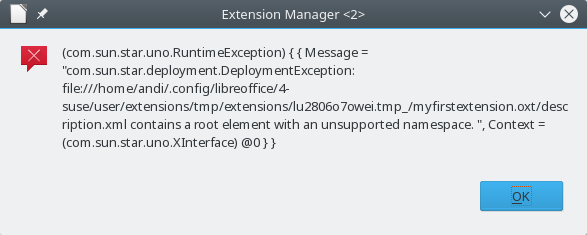
\includegraphics[width=0.7\linewidth]{pics/error_wrong_namedeclaration}
\captionof{figure}{Fehlermeldung wegen fehlerhafter Namespace-Deklaration}
\label{fig:error_wrong_namedeclaration}
\end{center}


\paragraph*{Identifier}$~~$\\

Als erste Ergänzung fügen wir in das Description-Tag einen sogenannten Identifier ein. Dies ist eine eindeutige Bezeichnung der Extension für den LibreOffice Extensionmanager. Es ist möglich, dass zwei inhaltlich bzw. auf Dateiebene identische Extensions vom Extensionmanager geladen werden, sofern sie unterschiedliche Identifier haben, nicht aber anders herum. Deshalb ist es wichtig, dass sie einen Identifier wählen, auf den nur Sie Zugriff haben bzw. der regelmäßig nur von Ihnen in dieser Form gewählt werden wird.

Der Identifier spielt dabei auch bei einem eventuell vorgesehenen Online-Update der Extension später eine wesentliche Rolle. Für unser Beispiel verwenden wir:
\begin{lstlisting}
<identifier value="org.mycompany.myfirstextension" />
\end{lstlisting}

\paragraph*{Version}$~~$\\

Als nächstes fügen wir die Angabe der Versionsnummer (Release-Nummer) der Extension in das Description-Tag als neues Tag ein:
\begin{lstlisting}
<version value="0.1" />
\end{lstlisting}
Als Werte (Value) kommen hier positive Zahlen in Betracht, die eine Versionsnummer der Extension darstellen können. Die Versions-Nummer kann aus lediglich einer positiven Ziffer (größer Null) oder einer Kolonne von mehreren durch Punkt getrennten Ziffern bestehen, z.B. 0.1.3. Das Benennungsschema sollte dabei den üblichen Geflogenheiten folgen. Die erste Ziffer bezeichnet insoweit Major-(Haupt-)Releases (mit eventueller Inkompatibilität zu bisherigen Haupt-Releases). Die zweite Ziffer steht für Änderungen im Sinne von Minor-Releases (mit kompatiblen Änderungen), während die dritte Ziffer Micro-Releases anzeigt (mit beispielsweise Fehlerbereinigungen).

\paragraph*{Plattform}$~~$\\

Eine LibreOffice Extension kann sowohl für alle Plattformen von LibreOffice lauffähig sein, als auch lediglich für einzelne. Dies wird über das Platform-Tag gesteuert. Wir gehen davon aus, dass die Extension für alle Plattformen geeignet ist und fügen daher folgendes Zeile ein:
\begin{lstlisting}
<platform value="all" />
\end{lstlisting}
Der Wert ("value") kann entweder eine oder mehrere Plattformen mit Komma getrennt enthalten. Beispielsweise in folgender Form:
\begin{lstlisting}
<platform value="windows_x86, linux_x86_64, linux_x86" /> 
\end{lstlisting} 
Die Extension kann nur installiert werden, wenn eine der angegebenen Plattformen dem laufenden Betriebssystem entspricht. Falls als Wert keine Plattform angegeben wird, kann die Extension unter keinem laufenden Betriebssystem installiert werden.
\begin{lstlisting}
<platform value=" " />
\end{lstlisting}
Der Extensionmanager von LibreOffice kann hier keine Plattform (Betriebssystem) ausfindig machen, auf dem die Extension lauffähig ist, und bricht daher die Installation ab.

Die folgende Tabelle listet alle möglichen Plattformen auf, die als Wert verwendet werden können, unabhängig davon, ob sie von LibreOffice unterstützt werden.\linebreak


\begin{tabular}{ |p{3cm}|p{9cm} | }
	
	\multicolumn{2}{l}{\textbf{Platform Token (Plattform-Schlüssel)}}\\
	\toprule
	\rowcolor{hellgrau}
	Token (Schlüssel)& Beschreibung\\
	\hline
	all   & Umfasst alle Plattformen\\
	\hline
    \verb|freebsd_x86|& FreeBSD Betriebssystem auf X86-Plattform\\
    \hline
    \verb|freebsd_x86_64|& FreeBSD Betriebssystem auf 64bit-Plattform\\
    \hline
    \verb|linux_arm_eabi|& (Aktuell nicht unterstützt) Linux Betriebssystem auf einer ARM-CPU unter Verwenden von "EABI"\\
    \hline
    \verb|linux_arm_oabi|& (Aktuell nicht unterstützt) Linux Betriebssystem auf einer ARM-CPU unter Verwenden von "OABI"\\
    \hline
    \verb|linux_ia64| &	Linux Betriebssystem auf einer ia64 CPU\\
    \hline
    \verb|linux_mips_eb| &	(Aktuell nicht unterstützt) Linux Betriebssystem auf einer MIPS CPU unter verwenden von 'EB' ABI\\
    \hline
    \verb|linux_mips_el| &	(Aktuell nicht unterstützt) Linux Betriebssystem auf einer MIPS CPU unter verwenden von 'EL' ABI.\\
    \hline
    \verb|linux_powerpc| &	Linux Betriebssystem auf einer POWERPC CPU.\\
    \hline
    \verb|linux_powerpc64| & (Aktuell nicht unterstützt) Linux Betriebssystem auf einer POWERPC 64bit CPU.\\
    \hline
    \verb|linux_s390| &	Linux Betriebssystem auf einer s390 CPU.\\
    \hline
    \verb|linux_s390x| & (Aktuell nicht unterstützt) Linux Betriebssystem auf einer s390x CPU.\\
    \hline
    \verb|linux_sparc| & Linux Betriebssystem auf einer SPARC CPU.\\
    \hline
    \verb|linux_x86| &	Linux Betriebssystem auf einer x86 CPU.\\
    \hline
    \verb|linux_x86_64| & Linux Betriebssystem auf einer x86 64 bit CPU\\
    \hline
    \verb|macosx_powerpc| &	Mac X Betriebssystem auf einer POWERPC CPU\\
    \hline
    \verb|macosx_x86| &	Mac X Betriebssystem auf einer x86 CPU\\
    \hline
    \verb|macosx_x86_64| & 	Mac X Betriebssystem auf einer x86-64 CPU\\
    \hline
    \verb|os2_x86| & OS/2 Betriebssystem auf einer x86 CPU\\
    \hline
    \verb|solaris_sparc| & 	Solaris Betriebssystem auf einer SPARC CPU\\
    \hline
    \verb|solaris_x86| & Solaris Betriebssystem auf einer x86 CPU\\
    \hline
    \verb|windows_x86| & Windows operating system running on a x86 CPU\\ 
    \bottomrule
\end{tabular}

\paragraph*{Rückwärtskompatibilität von Plattformen}$~~$\\
Teilweise wird ein LibreOffice-32-bit-Build auch auf 64-bit-Linux-Plattformen ausgeführt. In einem solchen Fall vergleicht der Extensionmanager die Plattform der Extension mit derjenigen, für die LibreOffice erstellt wurde. Die folgende Tabelle enthält einige Beispiele für Kombinationen und die jeweiligen Ergebnisse. 


\begin{tabular}{|p{3.0cm}|p{3.0cm}|p{3.0cm}|p{1.5cm}|}
	\hline \rowcolor{hellgrau} \rule[-2ex]{0pt}{5.5ex}  Extension Plattform & LibreOffice erstellt für Plattform & Plattform, auf der LibreOffice läuft  & Resultat \\
	\hline \rule[-2ex]{0pt}{5.5ex} \verb|Linux_x86 | & \verb|Linux_x86 | & \verb|Linux_x86 | & OK \\ 
	\hline \rule[-2ex]{0pt}{5.5ex} \verb|Linux_x86 | & \verb|Linux_x86 | & \verb|Linux_x86_64 | & OK \\ 
	\hline \rule[-2ex]{0pt}{5.5ex} \verb|Linux_x86 | & \verb|Linux_x86_64 | & \verb|Linux_x86_64 | & Scheitert \\ 
	\hline \rule[-2ex]{0pt}{5.5ex} \verb|Linux_x86_64 | & \verb|Linux_x86 | & \verb|Linux_x86_64 | & Scheitert \\ 
	\hline 
\end{tabular}
\paragraph*{Anzeigename der Extension}$~~$\\

Als nächstes fügen wir dem Description-Tag einen Namen hinzu, der im Extensionmanager angezeigt wird. Dieser Name kann auch für die einzelne Lokalisierungen vorgegeben werden. Der umschließende Tag lautet <display-name>.
Der angezeigte Name wird dann in einem oder mehreren <name>-Tags vorgegeben.

Sofern der <name>-Tag einen Zusatz bzgl. der Sprache (lang) enthält, wird dieser Text für die entsprechende Lokalisierung angezeigt. Ohne einen solchen Zusatz bzw. für andere Lokalisierungen ohne eigenen <name>-Tag wird der Standard bzw. die englische Version angezeigt. Für unsere Beispiel-Extension geben fügen wir dem Description-Tag folgendes hinzu:
\begin{lstlisting}
<display-name>
    <name lang="de">Meine erste LibreOffice Extension</name>
    <name lang="en">My first LibreOffice extension</name>
</display-name>
\end{lstlisting}

\paragraph*{Autor}$~~$\\

Nun fügen wir noch den Autor über das <publisher>-Tag der Description hinzu. In unserem Beispiel lautet der Tag für mich selbst folgendermaßen:
\begin{lstlisting}
<publisher>
   <name xlink:href="http://amantke.de/blog">Andreas Mantke</name>
</publisher>
\end{lstlisting}
Der <publisher>-Tag muss zumindest einen <name>-Tag haben. Letzterer Tag kann wieder für unterschiedliche Lokalisierungen über einen lang-Zusatz vorgegeben werden. Der <name>-Tag selbst enthält eine URL zusammen mit dem ggfs. lokalisierten Namen des Autors.

Die Datei description.xml sieht nun wie folgt aus:
\begin{lstlisting}
<?xml version="1.0" encoding="UTF-8"?>
<description
    xmlns="http://openoffice.org/extensions/description/2006"
    xmlns:xlink="http://www.w3.org/1999/xlink">

    <identifier value="org.mycompany.myfirstextension" />
    <version value="0.1" />
    <platform value="all" />

    <display-name>
        <name lang="de">
            Meine erste LibreOffice Extension</name>
        <name lang="en">
            My first LibreOffice extension</name>
    </display-name>
    <publisher>
        <name xlink:href="http://amantke.de/blog">
            Andreas Mantke</name>
    </publisher>    
</description>
\end{lstlisting}

\section{Meta-Informationen}

Eine LibreOffice Extension benötigt zumindest eine Datei manifest.xml, die weitere Verwaltungsinformationen enthalten kann. Ohne diese Datei ließe sich die Extension zwar installieren, aber eine Deinstallation würde scheitern mit einer Fehlermeldung wie im folgenden Bildschirmfoto.
\begin{center}
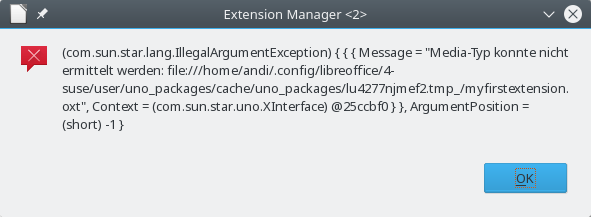
\includegraphics[width=0.7\linewidth]{pics/error_deinstallation_missing_manifest}
\captionof{figure}{Fehlermeldung wegen fehlender Datei manifest.xml beim Entfernen der Extension}
\label{fig:error_deinstallation_missing_manifest}
\end{center}

Wir legen dazu ein Unterverzeichnis \glqq META-INF\grqq~und in diesem eine neue Datei manifest.xml an. Die Datei bekommt zunächst nur folgenden Inhalt:
\begin{lstlisting}
<?xml version="1.0" encoding="UTF-8"?>
<manifest:manifest 
    xmlns:manifest="http://openoffice.org/2001/manifest">
</manifest:manifest>
\end{lstlisting}



\section{Erstellen der Extension-Datei}

Mit diesen ersten Versionen der Dateien description.xml und manfest.xml können wir nun eine Testversion der Extension-Datei erstellen und versuchen, die Extension noch ohne Funktionalität mit dem Extensionmanager zu installieren (und wieder zu deinstallieren)
Bei der Extension-Datei (*.oxt) handelt es sich um einen komprimierten Container. Um diesen zu erstellen, können Sie dem für die Test-Extension erstellten folgendes Python-Buildskript hinzufügen. Dieses Skript hat Björn Michaelsen erstellt. Es steht unter der Mozilla Public License (MPL) und ist beispielsweise hier zu finden: \url{https://gerrit.libreoffice.org/gitweb?p=sdk-examples.git;a=blob;f=BundesGit/build;h=4e29b2addb081599100c5e8b48c384bbfff427ca;hb=HEAD}

Das Skript setzt voraus, dass im Verzeichnis eine weitere Textdatei mit dem Namen extensionname.txt vorhanden ist, die den Namen der Extension enthält, hier den Text
\begin{lstlisting}
myfirstextension.oxt
\end{lstlisting}
Das Build-Skript mit dem Namen build sieht folgendermaßen aus:
\begin{lstlisting}
#!/usr/bin/env python
# This Source Code Form is subject to the terms of the 
# Mozilla Public License, v. 2.0. If a copy of the MPL was  
# not distributed with this file, You can obtain one at 
# http://mozilla.org/MPL/2.0/.

from zipfile import ZipFile
import os, os.path, sys
scriptdir = os.path.dirname(os.path.abspath(sys.argv[0]))
extensionname = open(
    os.path.join(scriptdir, 
        'extensionname.txt')).readlines()[0].rstrip('\n')
with ZipFile(extensionname, 'w') as tuesdayzip:
    os.chdir(scriptdir)
    for root, dirs, files in os.walk('.'):
        for name in files:
            if not name == extensionname:
                tuesdayzip.write(os.path.join(root, name)) 
\end{lstlisting}
Da das Skript in der Programm-Sprache Python geschrieben ist, müssen Sie darauf achten, dass die Einrückungen korrekt übernommen werden. Das Skript selbst rufen Sie später einfach mit
\begin{lstlisting}
python ./build
\end{lstlisting}
auf. Die Extension-Datei wird dadurch in dem Verzeichnis der Test-Extension erstellt.

\section{Erste Testinstallation der Extension}

Die gerade erstellte OXT-Datei installieren wir nun testweise mit dem Extensionmanager von LibreOffice. Wir starten dazu LibreOffice und wählen im Menü Extras den Eintrag "Extension Manager". In der sich öffnenden Dialogbox aktivieren wir die Schaltfläche "Hinzufügen" und navigieren in dem nun geöffneten Datei-Dialog zu der gerade erstellten OXT-Datei und bestätigen die Auswahl über die Schaltfläche "Öffnen". Die neue Extension sollte anschließend im Dialogfenster gelistet sein.
\begin{figure}
\centering
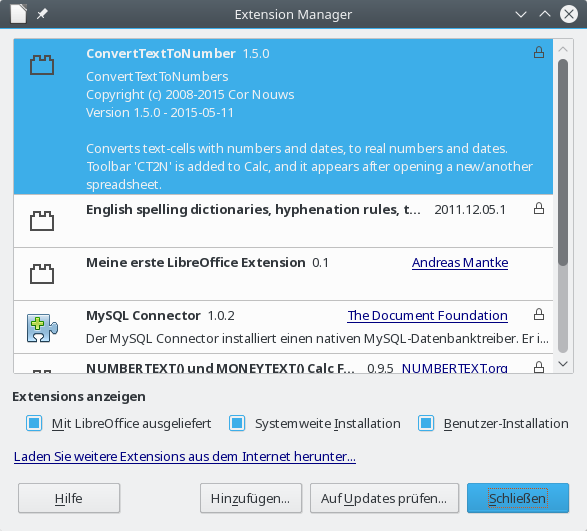
\includegraphics[width=0.7\linewidth]{pics/extensionmanager_extension_load01}
\caption[Extension Manager mit installierter Extension]{Der LibreOffice Extension Manager nach Installation der neuen Extension}
\label{fig:extensionmanager_extension_load01}
\end{figure}

Auf der rechten Seite des Eintrags für die neue Extension befindet sich der Name des Autors verbunden mit einem Link zu der URL, die in dem <name>-Tag innerhalb des <publisher>-Tags angegeben wurde. Dieser kann mit einem Mausklick im Standard-Browser aufgerufen werden.

Markieren Sie nun den neuen Eintrag im LibreOffice Extension Manager und deinstallieren Sie die Extension wieder über die nun angezeigte Schaltfläche "Entfernen". Die Extension sollte sich damit nach Bestätigen des folgenden Benutzerdialogs fehlerfrei entfernen lassen. Sofern dies nicht der Fall ist, könnte dies beispielsweise an einer fehlenden Datei manifest.xml (siehe dazu oben).

\section{Weitere Einträge in der Datei description.xml}

Auf der Abbildung im letzten Abschnitt ist zu sehen, dass für die Test-Extension im LibreOffice Extension Manager keine Grafik bzw. ein Logo angezeigt wird, wie beispielsweise für den MySQL Connector. Um ein solches Logo einzubinden, existiert der <icon>-Tag.

Erstellen Sie nun ein neues Unterverzeichnis \glqq images \grqq und anschließend eine neue Grafik bzw. ein neues Logo im Dateiformat PNG und der Dimension 42 mal 42 Pixel. Die Grafikdatei speichern Sie dann unter dem Namen \verb|"extensionicon_42.png"| im neuen Unterverzeichnis. Um das Logo einzubinden, fügen Sie dem <description>-Tag folgenden Eintrag hinzu:

\begin{lstlisting}
<icon>
    <default xlink:href="images/extensionicon_42.png" />
</icon>
\end{lstlisting}

In dem Tag hinter \glqq xlink:href \grqq wird die relative URL zu der Grafikdatei angegeben. Neben dem Link zu der Default-Grafik ist es möglich, parallel eine alternative Grafik mit hohem Kontrast, mit einem weiteren Tag anzugeben:
\begin{lstlisting}
<high-contrast xlink:href="(...)" />
\end{lstlisting}

\paragraph*{Minimale LibreOffice Version}$~~$\\

Es ist möglich, für die Extension eine minimale Version von LibreOffice anzugeben. Dies geschieht über den <dependencies>-Tag. Dieser Tag braucht eine Namespace-Deklaration, die hinter \glqq xmlns:lo \grqq erfolgt. Innerhalb der <dependencies>-Tag wird dann mit einem weiteren Tag die minimale LibreOffice-Version, für das Beispiel Version 4.2.

\begin{lstlisting}
<dependencies xmlns:lo=
    "http://libreoffice.org/extensions/description/2011">
    
    <lo:LibreOffice-minimal-version name="LibreOffice 4.2" 
        value="4.2"/>
    
</dependencies>
\end{lstlisting}

Die Vorgabe einer auch maximalen Version von LibreOffice, wie dies früher für OpenOffice.org möglich war, steht nicht mehr zur Verfügung. Der Tag für die Angabe der minimalen LibreOffice-Version erfordert neben der Übergabe des Wertes (\glqq value \grqq ) mit der Nummer des Releases (nur zweistellig, nicht ein etwaiges Micro-Release) auch die Vorgabe des Namens als Zeichenkette. Für die Anzeige der Meldung über die minimal erforderliche LibreOffice-Version im Extension Manager wird allerdings nur auf das angegebene Value zurückgegriffen.

\paragraph*{Beschreibung der Extension}$~~$\\

Der Extension kann eine Erläuterung Ihrer Funktionsweise über den <extension-description>-Tag hinzugefügt werden, wobei dieser mehrere Lokalisierungen dieser Beschreibung aufzunehmen.

Hierzu legen wir zunächst ein weiteres Unterverzeichnis \glqq description \grqq und darin zwei neue -zunächst leere Textdateien \verb|"description_de.txt"| und \verb|"description_en.txt"| an. Diese können später mit Informationen in deutscher und englischer Sprache befüllt werden. Wir binden diese beiden Beschreibungsdateien über folgende Ergänzung des <description>-Tag ein:
\begin{lstlisting}
<extension-description>
    <src xlink:href="description/description_en.txt" 
        lang="en" />
    <src xlink:href="description/description_de.txt" 
        lang="de" />
</extension-descritption>
\end{lstlisting}

Der in ihnen abgelegte Text wird nach der Installation im Extension Manager als Erläuterung angezeigt. Er sollte daher möglichst kurz und präzise formuliert werden und gegebenenfalls für ausführlichere Informationen auf eine externe Ressource (z.B. eine Webseite oder ein Wiki) verweisen.

Die Bezeichner für die Lokalisierung richten sich nach \href{https://tools.ietf.org/html/rfc3066}{RFC 3066}. Es sind daher sowohl Lokalisierungsbezeichner in der zuvor benutzten Form als auch spezifischere zulässig wie beispielsweise:
\begin{lstlisting}
<src (...) lang="en-GB" />
<src (...) lang="en-US" />
\end{lstlisting}

\paragraph*{Release Notes}$~~$\\

Es ist zwar möglich, in der Datei description.xml ein Tag für Release-Notes vorzugeben, allerdings hat dies für den Anwender keinen praktischen Nutzen, da ihm die Verbindung zu einer in dem <release-notes>-Tag eingestellten Verbindung zu einer URL im Extension Manager nicht angezeigt wird. Sofern für den Anwender wichtige Informationen zur Funktionsweise der Extension und zu Änderungen des oder der Release angezeigt werden sollten, eignet sich daher allein der zuvor beschriebene <description>-Tag und eine darin verlinkte externe Ressource am besten.

\paragraph*{Registration / Lizenz}$~~$\\

Das Registration-Element ermöglicht im Moment allein die Vorgabe der Lizenz der Extension, wobei auch hier wieder die Möglichkeit der parallelen Übermittlung von unterschiedlichen Lokalisierungen besteht.

Das <registration>-Element enthält ein <simple-license>-Element, welches wieder für jede Lokalisierung ein <license-text>-Element enthält. Das <simple-license>-Element enthält ein notwendiges Attribut \glqq accept-by \grqq . Optional sind zwei weitere Attribute in diesem Element möglich: \glqq suppress-on-update\grqq~ und \glqq suppress-if-required\grqq .\\

\begin{tabular}{|p{3.5cm}|p{8.3cm}|}
	\hline \rowcolor{hellgrau} \rule[-3ex]{0pt}{5.5ex}  Attribut & Beschreibung \\
	\hline \rule[-3ex]{0pt}{5.5ex} accept-by & Erforderlich. Der Wert kann entweder \glqq user\grqq~ oder \glqq admin\grqq~ sein. \glqq user\grqq~ bedeutet, dass jeder Benutzer der Lizenz zuzustimmen hat. Dies heißt dann, dass die Extension nur vom Benutzer und nicht vom Administrator als systemweite (shared) Extension installiert werden kann. Sofern der Wert \glqq admin\grqq~ gesetzt ist, kann die Extension auch als shared (geteilt / systemweit) installiert werden. In diesem Fall muss lediglich die Person, die die Extension installiert, der Lizenz zustimmen. Die einzelnen Benutzer werden nicht gefragt, ob sie die Lizenz akzeptieren. Sie können die Extension einfach benutzen.\\
	\hline \rule[-3ex]{0pt}{5.5ex}	suppress-on-update & Optional. Falls das Attribut nicht gesetzt ist, wird als Wert \glqq false\grqq~ angenommen. Sofern das Attribut mit dem Wert \glqq true\grqq~ vorgegeben ist, wird bei einem Update der Extension (gleiche ID, aber eventuell andere Version) der Lizenzdialog nicht erneut angezeigt.\\
	\hline \rule[-3ex]{0pt}{5.5ex}	suppress-if-required & Optional. Falls das Attribut nicht gesetzt ist, wird als Wert \glqq false\grqq~ angenommen. Der Wert \glqq true\grqq~ weist darauf hin, dass der Lizenzdialog während der Installation nicht angezeigt wird, sofern dies gewünscht wird. Dies kann dann durch den Schalter  \verb|--suppress-license| von unopkg vorgegeben werden und wird implizit für mitgelieferte (gebündelte) Extensions vorausgesetzt.\\
	\bottomrule
	
\end{tabular}

\bigskip
\bigskip
Legen Sie nun ein weiteres Unterverzeichnis \glqq registration\grqq~ und darin die Textdateien \verb|"license_de.txt"| und \verb|"license_en.txt"| an. Es reicht zunächst, wenn die Dateien existieren, auch wenn sie aktuell noch keinen Inhalt haben. Ihr späterer Inhalt wird, sofern nicht in der Einstellung unterdrückt, dem Benutzer im Installationsdialog angezeigt. In dem Dialog wird dann abgefragt, ob er die Lizenz akzeptiert.

\begin{lstlisting}
<registration>
    <simple-license accept-by="admin">
        <license-text xlink:href="registration/license_de.txt" 
            lang="de" />
        <license-text xlink:href="registration/license_en.txt" 
            lang="en" />
    </simple-license>
</registration>
\end{lstlisting}

Die Datei description.xml hat mit den weiteren vorgenommenen Ergänzungen nun folgenden Inhalt:

\begin{lstlisting}
<?xml version="1.0" encoding="UTF-8"?>
<description
    xmlns="http://openoffice.org/extensions/description/2006"
    xmlns:xlink="http://www.w3.org/1999/xlink">

    <identifier value="org.mycompany.myfirstextension" />
    <version value="0.1" />
    <platform value="all" />
    <display-name>
        <name lang="de">
            Meine erste LibreOffice Extension</name>
        <name lang="en">
            My first LibreOffice extension</name>
    </display-name>
    <publisher>
        <name xlink:href="http://amantke.de/blog">
            Andreas Mantke</name>
    </publisher>
    <icon>
        <default xlink:href="images/extensionicon_42.png" />
    </icon>
    <dependencies xmlns:lo=
        "http://libreoffice.org/extensions/description/2011">
        <lo:LibreOffice-minimal-version name="LibreOffice 4.2" 
            value="4.2"/>
    </dependencies>
    <extension-description>
        <src xlink:href="description/description_en.txt" 
            lang="en" />
        <src xlink:href="description/description_de.txt" 
            lang="de" />
    </extension-description>
    <registration>
        <simple-license accept-by="admin">
            <license-text xlink:href="registration/license_de.txt" 
                lang="de" />
            <license-text xlink:href="registration/license_en.txt" 
                lang="en" />
        </simple-license>
    </registration>
</description>

\end{lstlisting}

\chapter{Auslieferung von Inhalten mit Extensions}

MIt einer LibreOffice Extension lassen sich verschiedene Arten von Inhalten dem Standard-Programm hinzufügen. So ist es beispielsweise möglich, der Gallery, einem Verwaltungsmodul für Grafiken, Zeichnungen, Musik und andere Multimediadateien, neue Bereiche und Dateien hinzuzufügen. Wie Sie eine solche Extension erstellen, soll im folgenden Abschnitt erläutert werden.

\section{Gallery-Extension}

Bevor wir eine Gallery-Extension erstellen können, müssen wir zunächst mit LibreOffice ein entsprechendes neues Gallery-Thema erstellen, das wir dann mit neuen Inhalten (z.B. Grafiken) befüllen und die entstandenen Dateien exportieren.

\subsection{Neues Gallery-Thema erstellen}

Beginnen wir also mit dem Erstellen eines neuen Gallery-Themas in LibreOffice. Starten Sie das Programm. Die Gallery rufen Sie über das Menü \glqq Ansicht\grqq~und den dortigen Eintrag \glqq Gallery\grqq~auf. Die Gallery wird damit in der Seitenleiste geöffnet (früher wurde sie oberhalb des Bearbeitungsfensters unterhalb der Menüleiste angezeigt). Im oberen Bereich werden die vorhandenen Themen in Ihrem LibreOffice angezeigt Erstellen Sie nun über die Schaltfläche \glqq Neues Thema\grqq~und den folgenden Dialog ein solches Thema. Auf dem ersten Register (\glqq Allgemein\grqq) des Dialogs geben Sie einen Namen für das Thema vor. Sofern Sie bereits zuvor Grafiken, Zeichnungen oder Multimedia-Dateien erstellt haben, können Sie diese über das Register \glqq Dateien\grqq~direkt dem Thema hinzufügen. Wir nennen das Thema \glqq Tiere\grqq~ nennen, da wir einige Grafiken mit offenen Lizenzen aus dem Openclipart-Projekt in unserer Beispiel-Extension in der LibreOffice-Gallery verfügbar machen wollen.

Die Grafiken auf der Seite von OpenClipart (https://openclipart.org) werden dort unter Public Domain veröffentlicht. OpenClipart verwendet dazu die Creative Commons Zero 1.0 Public Domain License \linebreak(https://creativecommons.org/publicdomain/zero/1.0/).

Für unser gerade erstelltes Tier-Thema  in der Gallery laden wir mehrere Tiergrafiken von der OpenClipart-Webseite möglichst im Vektorformat (SVG) herunter, z.B. einen Elefanten (Elephant), einen Tiger und einen Wolf.

\chapter{Konfigurationseinstellungen mit einer Extension verteilen}

\end{document}

